
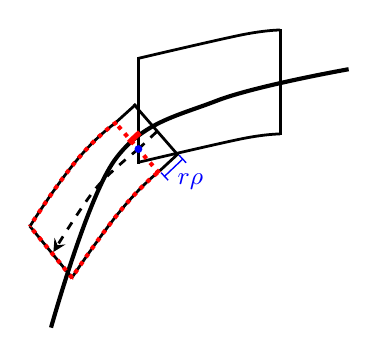
\begin{tikzpicture}[scale=6]
    % Draw smooth curved path
    \draw[color=black, line width = 1.5] plot[smooth, tension = .6] coordinates{
         (.195, 0.31) (0.33, 0.665) (0.545, 0.79) (.825, .857)  
    }; 
    
   
    % Draw the curved pipe (thick tube-like shape)
    \draw[black, line width = 1, rounded corners=0.02cm] 
        (.68,.718) -- (.68,.942);
    \draw[black, line width = 1, rounded corners=0.02cm] 
        (.38,.657) -- (.38,.882);
 
    \draw[color=black, line width = 1] plot[smooth, tension = .6] coordinates{
        (.38, .66) (.60, .71) (.68, .72)  
    }; 
    
    \draw[color=black, line width = 1] plot[smooth, tension = .6] coordinates{
        (.38, .88)  (.60, .93) (.68, .94)  
    }; 


         \draw[dashed, line width = 1] 
        (.38,.688) -- (.419,.725); % Reduced the length but kept the slope

    % Lowered dashed tangent arrow
    \draw[line width=1pt,black,-stealth, dashed] plot[smooth, tension = .6] coordinates{
        (0.38, .688) (0.29, .605)  (0.2, 0.47) % Shifted y-values downward
    }; 

         \draw[color=blue,, line width = .5] 
        (.428,.638) -- (.443,.622); % Reduced the length but kept the slope     
         \draw[color=blue,, line width = .5] 
        (.466,.675) -- (.481,.659); % Reduced the length but kept the slope     
         \draw[color=blue,, line width = .5] 
        (.435,.63) -- (.474,.667); % Reduced the length but kept the slope
        % blue circle node at (.38, .688)
    \node[blue, inner sep=1pt] at (0.49, .62) {{\small$r\rho$}};


     % Draw shorter middle segment with same slope
    \draw[ line width = 1] 
        (.464,.675) -- (.37,.783); % Reduced the length but kept the slope
    \draw[ line width = 1] 
        (.24,.415) -- (.15,.525); % Lowered slightly
    \draw[ line width = 1] 
        (.464,.678) -- (.423,.64); % Reduced the length but kept the slope
    \draw[ line width = 1] 
        (.375,.783) -- (.333,.745); % Reduced the length but kept the slope


    
       % Lowered curved tube around the arrow
    \draw[color=black, line width = 1] plot[smooth, tension = .9] coordinates{
        (0.42, .6375) (0.34, .555) (0.238, .414)  % Shifted downward
    }; 
    
    \draw[color=black, line width = 1] plot[smooth, tension = .9] coordinates{
        (0.334, .745) (0.25, .665) (0.15, .524)  % Shifted downward
    }; 
       
     % Draw shorter middle segment with same slope
    \draw[red, line width = 1.5,dotted] 
        (.424,.637) -- (.33,.745); % Reduced the length but kept the slope
    \draw[red, line width = 1.5,dotted] 
        (.24,.415) -- (.15,.525); % Lowered slightly



 % Lowered curved tube around the arrow
    \draw[color=red, line width = 1.5,dotted] plot[smooth, tension = .9] coordinates{
        (0.42, .6375) (0.34, .555) (0.238, .414)  % Shifted downward
    }; 
    
    \draw[color=red, line width = 1.5,dotted] plot[smooth, tension = .9] coordinates{
        (0.334, .745) (0.25, .665) (0.15, .524)  % Shifted downward
    }; 
    \draw[color=red, line width = 2] plot[smooth, tension = .9] coordinates{
        (0.383, .723) (0.37, .711) (0.36, .701)  % Shifted downward
    }; 
    
        % blue circle node at (.38, .688)
    \node[circle, fill=blue, inner sep=1pt] at (0.38, .688) {};
 

\end{tikzpicture}
